\documentclass[tikz,border=10pt]{standalone}
\begin{document}
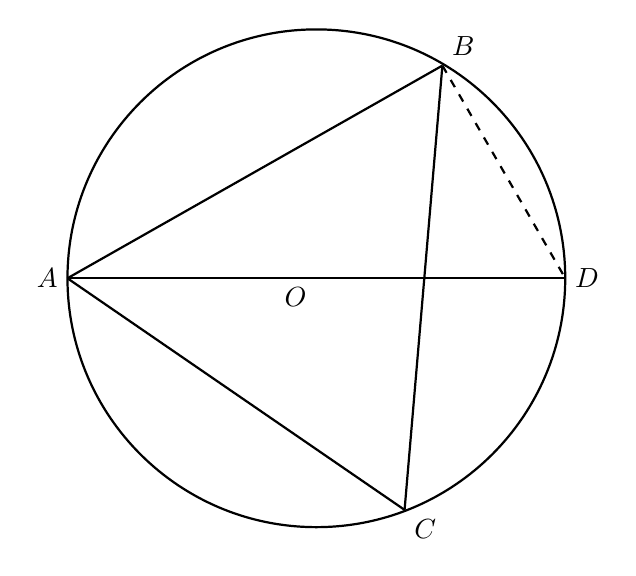
\begin{tikzpicture}[scale=0.02]
  \coordinate (O) at (0,0);
  \coordinate (A) at (-158,0);
  \coordinate (D) at (158,0);
  \coordinate (B) at (80,135);
  \coordinate (C) at (56,-147);

  \draw[thick] (O) circle (158);
  \draw[thick] (A) -- (B);
  \draw[thick] (B) -- (C);
  \draw[thick] (A) -- (C);
  \draw[thick] (A) -- (D);
  \draw[thick,dashed] (B) -- (D);

  \fill (O) circle (6pt);

  \node[above right] at (B) {$B$};
  \node[left] at (A) {$A$};
  \node[right] at (D) {$D$};
  \node[below left] at (O) {$O$};
  \node[below right] at (C) {$C$};
\end{tikzpicture}
\end{document}
